\chapter{Heroku}

\section{Introdução}
O Heroku é uma plataforma de computação em nuvem conhecida no mercado, com a possibilidade de subir aplicações nas linguagens Ruby, Node.js, Java, Python, Clojure, Scala, Go e PHP. O grande destaque do Heroku está na facilidade em subir uma aplicação com facilidade e de maneira gratuita, o que possibilita testar e validar ideias básicas antes de escalar de fato.

A estrutura básica do Heroku funciona com o uso de \textit{dynos}, que servem tanto para hospedar sua aplicação principal quanto máquinas auxiliares para serviços externos e/ou paralelos. Porém, recentemente o Heroku disponibilizou também a estrutura de \textit{containers} em Docker (tecnologia de gerenciamento de \textit{containers}) (assim como seus principais concorrentes), gerando maior flexibilidade para o serviço.

\section{Funcionamento básico}

\begin{figure}[h!]
  \centering
  \includegraphics[scale=0.20]{imagens/heroku_architecture.eps}
  \caption{Arquitetura Básica do Heroku\cite{safariheroku}}
\end{figure}

O funcionamento do Heroku consiste no uso de \textit{dynos} para hospedar as aplicações e nos \textit{routers} para tratar e encaminhas as requisições dos usuários. Além disso, o próprio Heroku disponibiliza extensões para gerenciar sua aplicação, como por exemplo o gerenciador de IP estático, ou o banco de dados necessário para a aplicação.

Um \textit{dyno} é um \textit{container} pronto, com 512MB de memória RAM, responsável por abrigar uma ou mais instâncias de sua aplicação, permitindo escalabilidade e tolerância de erros. Além disso, os \textit{dynos} permitem rodas tarefas de sua aplicação à parte, como filas, requisições assíncronas, entre outros.

Já os \textit{routers} são responsáveis por gerenciar os acessos dos usuários às aplicações correspondentes, dado que não é padrão do Heroku estruturar IP estático para cada \textit{dyno}. Ou seja, a estrutura é responsável por fazer sua aplicação funcionar corretamente, sem acessar aplicações alheias.

\begin{figure}[h!]
  \centering
  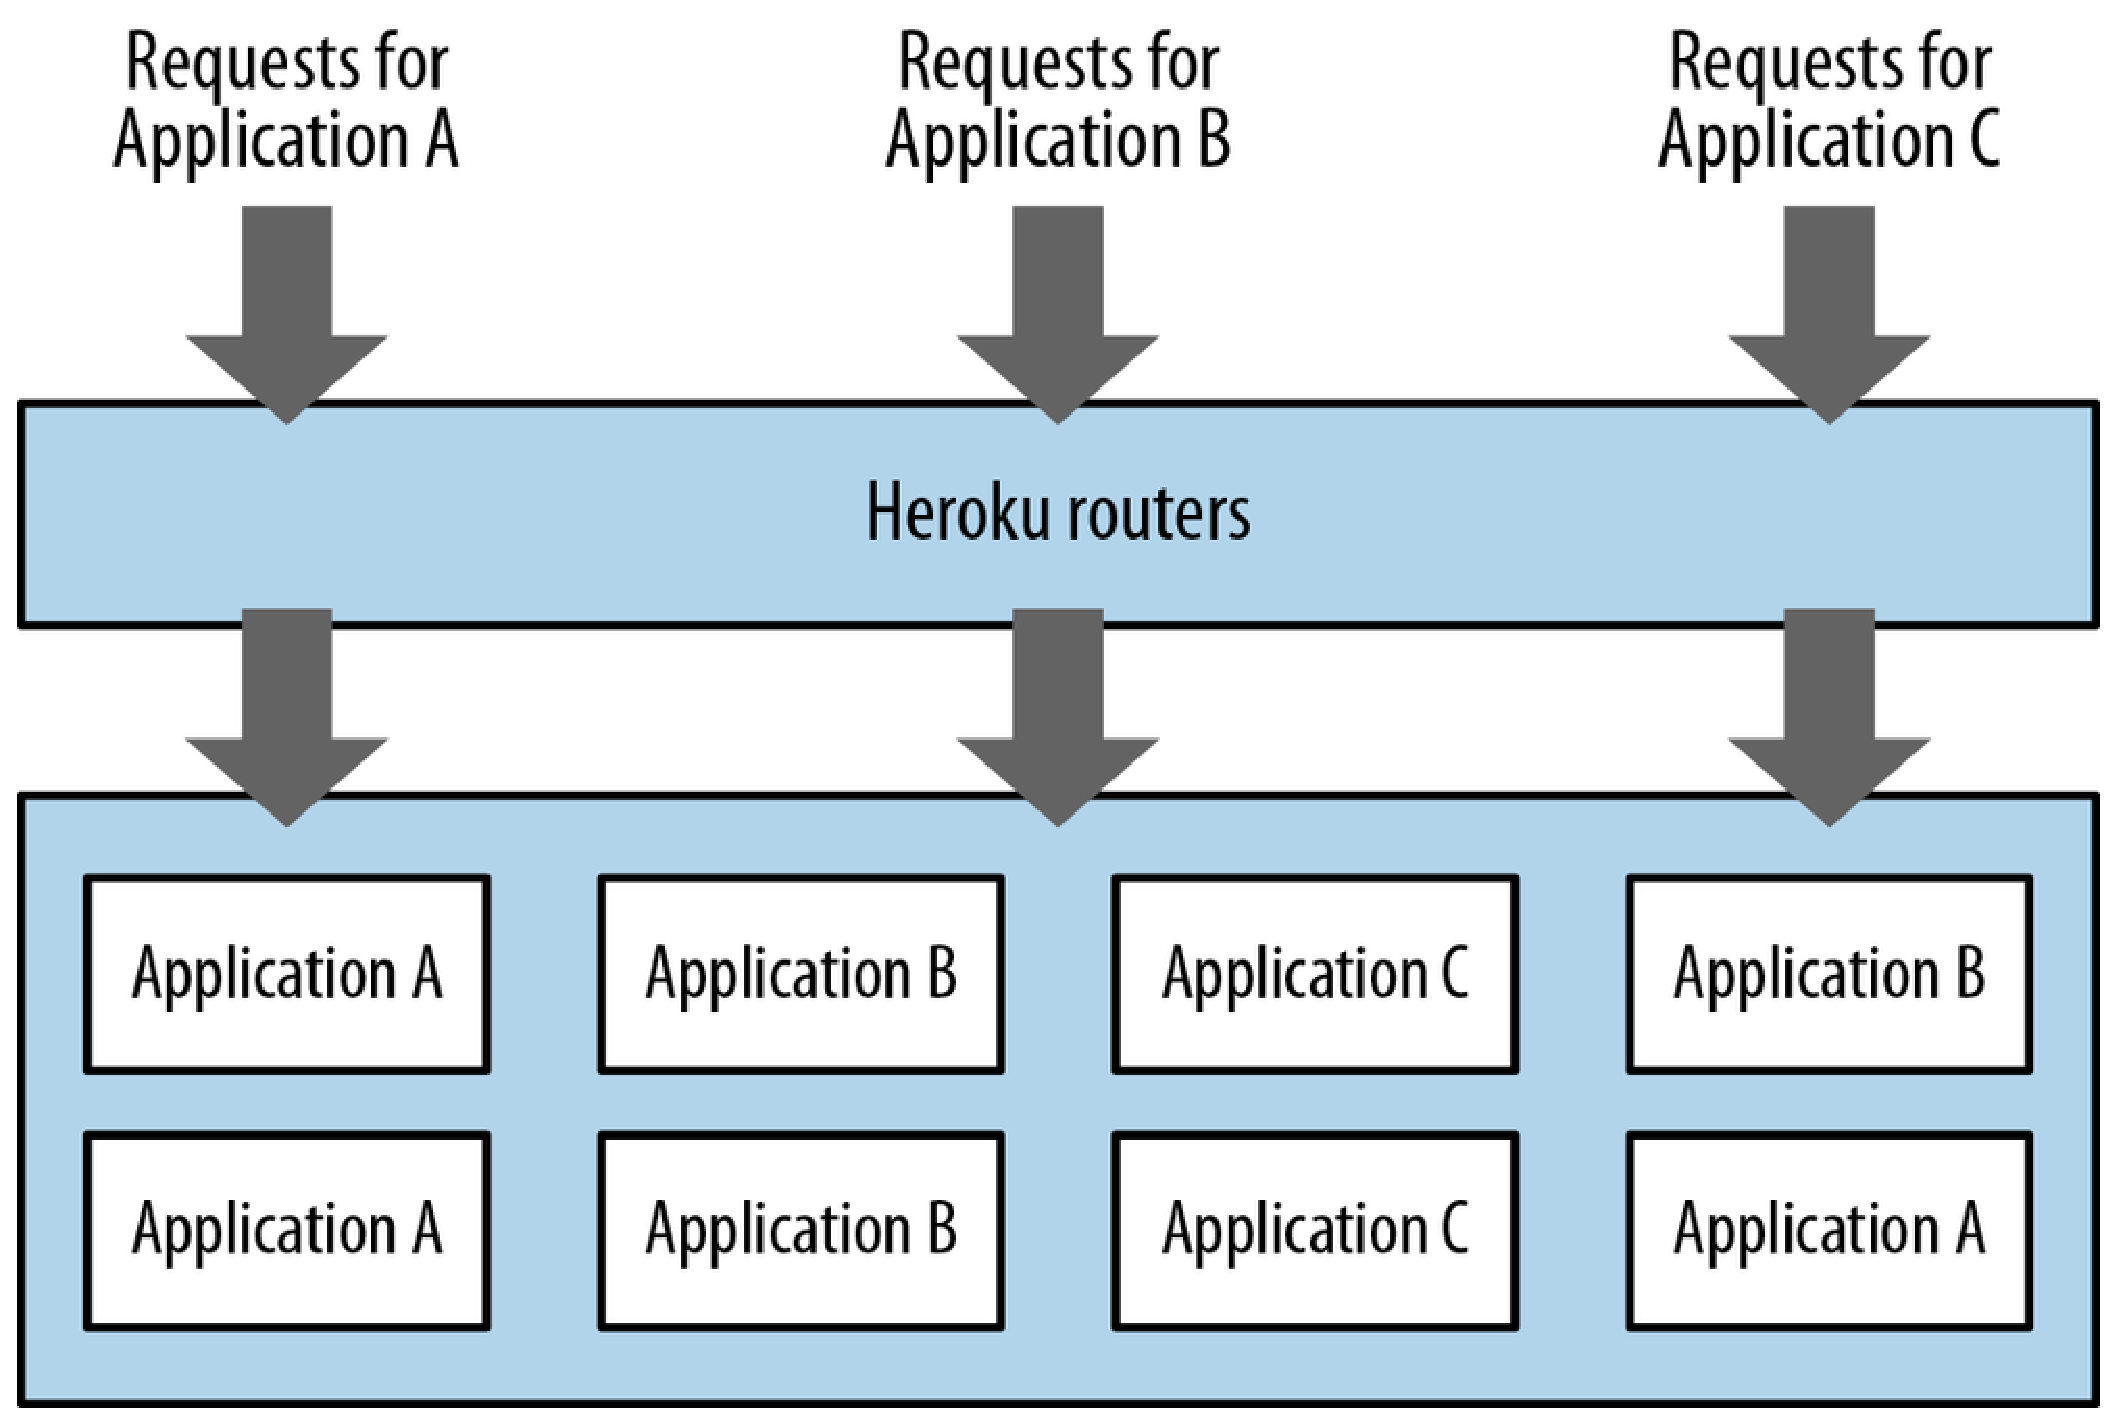
\includegraphics[scale=0.20]{imagens/heroku_router_dynos.eps}
  \caption{Ligação entre \textit{router} e \textit{dynos} do Heroku\cite{safariheroku}}
\end{figure}

Graças a essa estrutura, é possível, com facilidade, gerenciar versionamento e escalar a aplicação de maneira horizontal, com novos \textit{dynos} gerenciados pelo \textit{router}, dando uma popularidade considerável ao Heroku, em especial nas aplicações onde velocidade de validar hipóteses é o principal foco.

\section{Tarifação}

O Heroku possui um diferencial em relação à tarifação: possui um plano básico gratuito que possibilita testar aplicações de maneira fácil e sem dificuldades de expansão. Essencialmente, a cobrança do Heroku ocorre via uso de seus \textit{dynos}-hora. Além disso, há a cobrança pelas extensões usadas dentro da aplicação, onde, no geral, há um plano gratuito de testes ou até para projetos pequenos funcionarem com tranquilidade sem necessidades de escalabilidade.

Para qualquer usuário do Heroku, é disponibilizado um pacote de 750 \textit{dynos}-hora durante um mês, ou seja, uma aplicação gratuita usando um simples \textit{dyno} pode durar tranquilamente. Além disso, o Heroku de uso gratuito limita o tempo em que um \textit{dyno} fica ligado de maneira ociosa: passando trinta minutos desde a última requisição feita pelo cliente (e repassada pelo \textit{router}), o \textit{dyno} é derrubado, sendo religado após uma nova requisição.

\begin{figure}[h!]
  \centering
  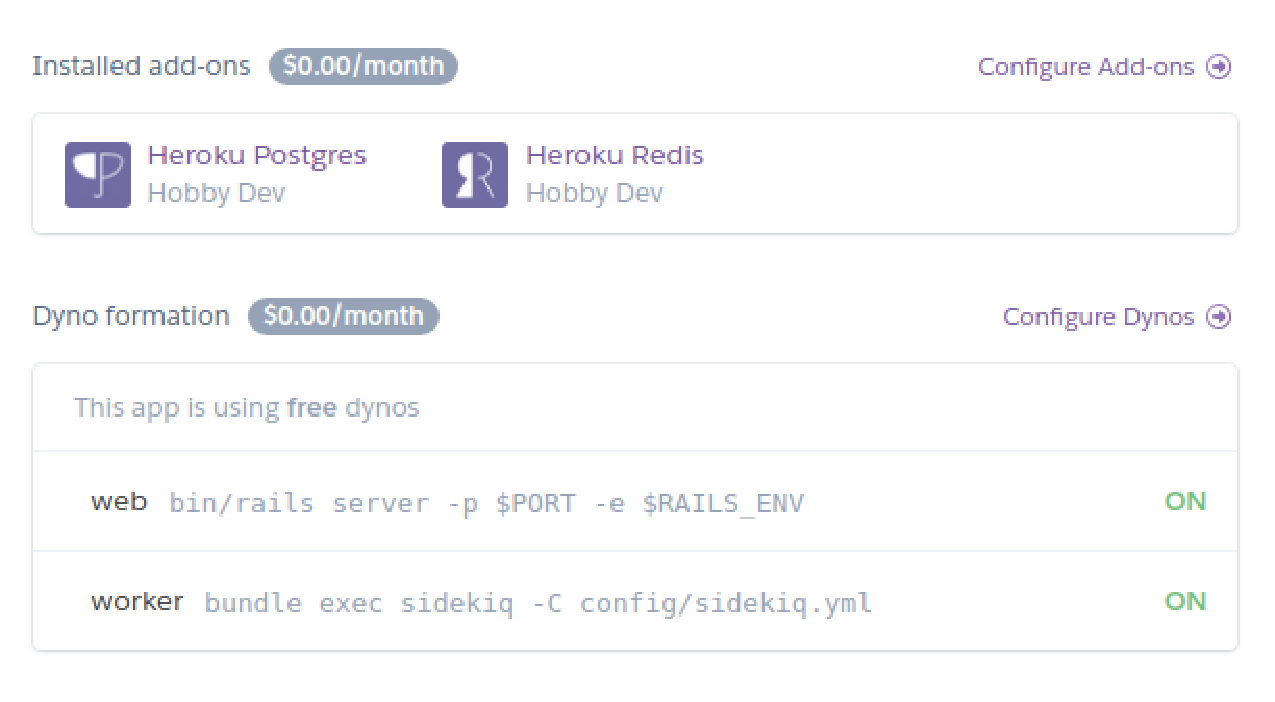
\includegraphics[scale=0.75]{imagens/heroku_dashboard.eps}
  \caption{Exemplo do \textit{Dashboard} do Heroku com seus recursos}
\end{figure}

Além da cobrança do uso dos \textit{dynos}, há também a cobrança para cada extensão utilizada por sua aplicação, o que de fato encarece o custo final para escalar uma aplicação. Por exemplo, o banco de dados relacional padrão do Heroku é gratuito até certo limite de dados, passando desse limite, há a extensão do plano que permite, além de mais dados armazenados, aumenta o fluxo possível de acesso ao banco.

\section{\textit{Containers}}

Recentemente, o Heroku possibilitou em seu catálogo de soluções o uso de estruturas isoladas customizadas: os \textit{containers}. \textit{Containers}, segundo o site do Docker\cite{dockercontainer} (em inglês):

\begin{citacaoLonga}
  A container image is a lightweight, stand-alone, executable package of a piece of software that includes everything needed to run it: code, runtime, system tools, system libraries, settings.
\end{citacaoLonga}

Ou seja, são imagens autossuficientes e virtualizadas que permitem rodar aplicações prontas nos mais diversos dispositivos, nos moldes da virtualização.

O Heroku possibilitou, em 2017, uma maneira eficiente de receber \textit{containers} em seu serviço, com o \textbf{Heroku Container Registry}\cite{herokucontainerregistry}. Esse serviço facilita colocar em produção as máquinas isoladas contruídas com o uso do \textit{Docker}, aumentando as possibilidades de operação com a plataforma. A tarifação do serviço segue o mesmo padrão do Heroku tradicional, dado o fato de que \textit{dynos} são uma espécie de \textit{containers}.

\section{Conclusão}

O Heroku é uma solução que se destaca pela velocidade e facilidade de colocar uma ideia em produção, de maneira gratuita, com possibilidades eficientes de escalabilidade. Porém, financeiramente, não é a melhor solução, com uma tarifação elevada para escalar a aplicação. Além disso, sua estrutura atende apenas aplicações prontas, não permitindo outras estruturas avançadas como o uso de \textit{containers}, sendo incorporado ao catálogo de produtos recentemente.
